\section{Plateau model (model ID: 15)}
The Plateau model (fig.~\ref{fig:15_schematic}) is a conceptualization of the perceived dominant processes in a typical Western European plateau \citep{Savenije2010}. It belongs to a 3-part topography driven modelling exercise, together with a wetland and hillslope conceptualization. Each model is provided in isolation here, because they are well-suited for isolating specific model structure choices. It has 2 stores and 8 parameters ($F_{max}$, $D_p$, $S_{u,max}$, $lp$, $p$, $T_p$, $C$ and $K_p$). The model aims to represent:

\begin{itemizecompact}
\item Stylized interception by vegetation;
\item Evaporation controlled by a wilting point and moisture constrained transpiration;
\item Separation between infiltration and infiltration excess flow;
\item Capillary rise and linear relation runoff from groundwater.
\end{itemizecompact}

\subsection{MARRMoT model name}
m\_15\_plateau\_8p\_2s \\

% Equations
\subsection{Model equations}

% Model layout figure
{ 																	% This ensures it doesn't warp text further down
\begin{wrapfigure}{l}{6cm}
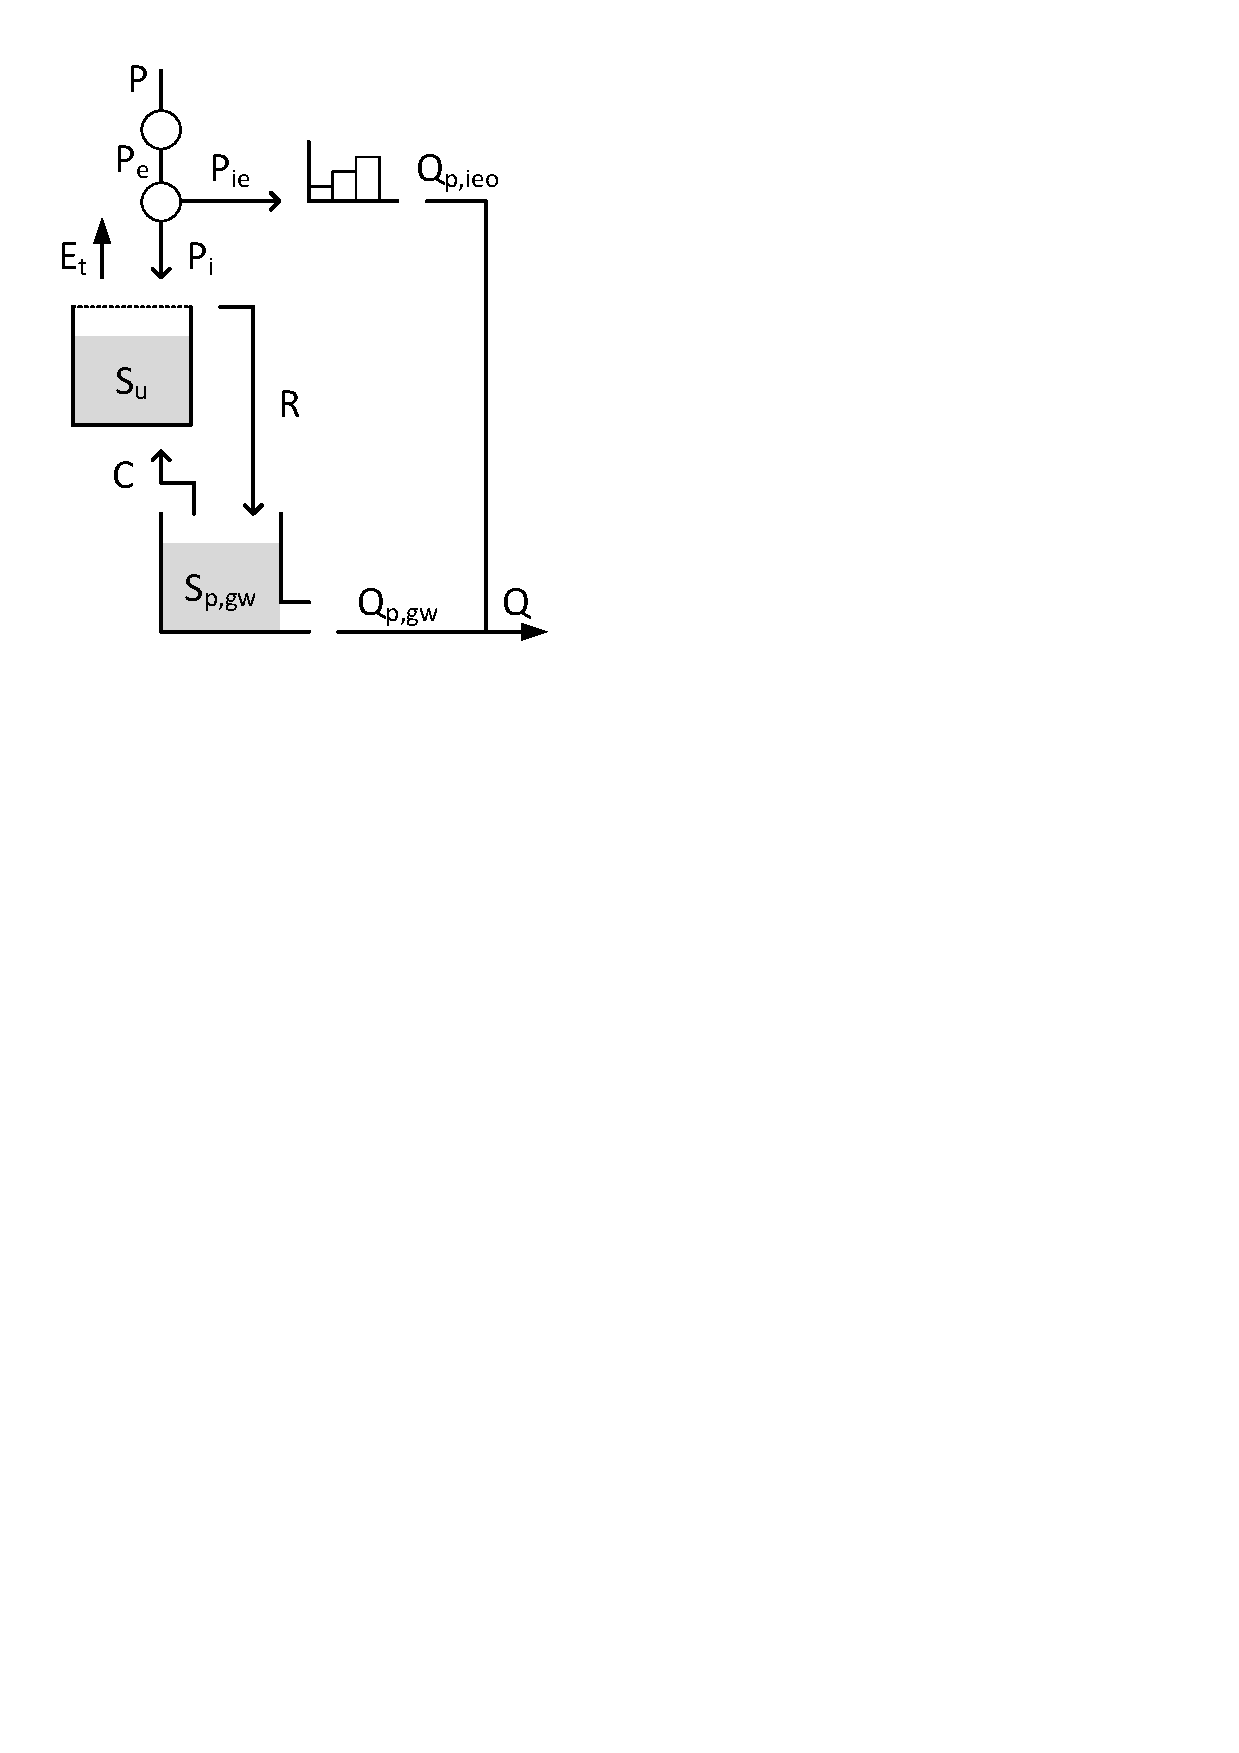
\includegraphics[trim=1cm 19cm 9cm 1cm,width=7cm,keepaspectratio]{./AppA_files/15_schematic.pdf}
\caption{Structure of the Plateau model} \label{fig:15_schematic}
\end{wrapfigure}

\begin{align}
	\frac{dS_u}{dt} &= P_i+C-E_t-R \\
	P_i &= min(P_e,F_{max})\\
		& = min\left(max(P-D_p,0),F_{max}\right)\\
	C &= c.\\
	E_t &= E_p*max\left(p\frac{S_u-S_{wp}}{S_{u,max}-S_{wp}},0\right)\\
	R &=	\begin{cases}
		P_i+C, & \text{if } S_u = S_{u,max} \\
		0, & \text{otherwise}\\
	\end{cases}
\end{align}

Where $S_u$ is the current soil water storage [mm]. Incoming precipitation P [mm/d] is reduced by interception $D_p$ [mm/d], which is assumed to evaporate before the next precipitation event. $P_e$ is further divided into infiltration $P_i$ [mm/d] based on the maximum infiltration rate $F_{max}$ [mm/d] and infiltration excess $P_{ie} = P_e-P_i$ [mm/d]. $C$ is capillary rise from ground water [mm/d], given as a constant rate.

 } % end of wrapfigure fix 

\noindent Evaporation from soil moisture $E_t$ [mm/d] occurs at the potential rate $E_p$ when $S_u$ is above the wilting point $S_{wp}$ [mm] (here defined as $S_{wp} = lp*S_{u,max}$) and is further constrained by coefficient $p$ [-], which is between 0 and 1. Storage excess $R$ [mm/d] flows into the groundwater. 

\begin{align}
	\frac{dS_{p,gw}}{dt} &=R-C-Q_{p,gw} \\
	Q_{p,gw} &= K_p*S_{p,gw}
\end{align}

Where $S_{p,gw}$ is current groundwater storage [mm]. Groundwater flow $Q_{p,gw}$ [mm/d] depends linearly on current storage $S_{p,gw}$ through parameter $K_p$ [$d^{-1}$]. Total flow $Q_t$ is the sum of $Q_{p,gw}$ and $Q_{p,ieo}$, the latter of which is $P_{ie}$ lagged over $T_p$ days.

\subsection{Parameter overview}
% Table generated by Excel2LaTeX from sheet 'Sheet1'
\begin{table}[htbp]
  \centering
    \begin{tabular}{lll}
    \toprule
    Parameter & Unit  & Description \\
    \midrule
    $F_{max}$ & $mm~d^{-1}$ & Maximum infiltration rate \\
    $D_p$ & $mm~d^{-1}$ & Interception evaporation  \\
    $S_{u,max}$ & $mm$  & Maximum soil moisture storage \\
    $lp$  & $-$   & Wilting point as fraction of $S_{u,max}$ \\
    $p$   & $-$   & Evaporation reduction factor \\
    $T_p$ & $d$   & Unit Hydrograph time base \\
    $C$   & $mm~d^{-1}$ & Capillary rise \\
    $K_p$ & $d^{-1}$ & Runoff coefficient \\
    \bottomrule
    \end{tabular}%
  \label{tab:addlabel}%
\end{table}%


